\documentclass{article}

\usepackage{a4wide}
\usepackage[utf8]{inputenc}
\usepackage[T1]{fontenc}
\usepackage[french]{babel}
\usepackage[babel=true]{csquotes} % guillemets français
\usepackage{graphicx}
\usepackage{float}
\graphicspath{{Images/}}
\usepackage{color}
\usepackage{hyperref}
\hypersetup{colorlinks,linkcolor=,urlcolor=blue}
\usepackage{amsmath}
\usepackage{amssymb}

\usepackage[
backend=biber,
style=alphabetic,
sorting=ynt
]{biblatex}

\addbibresource{ProjetDevMob.bib}

\title{Développement Mobile : \\ Jeu Snake}
\author{Sinama Richard, l3 Informatique \\ LE LIDEC Tristan, L3 Informatique}
\date{\today}

\begin{document}

\maketitle % pour écrire le titre

%% Le résumé:
\begin{abstract}
Dans notre rapport, nous verrons pas de façon structuré les différentes parties abordé lors de la création de notre projet. D'une part les approches selon le language, la structure de notre projet et pour finir les différents problème que nous aillons rencontré durant notre création d'application mobile.
\end{abstract}

\tableofcontents

\newpage

\section{Introduction}
\label{section:intro} % pour faire référence à la section ailleurs (\ref{...} voir plus bas)
Dans le cadre de l'UE Développement Mobile, nous avons eu à réaliser une application sur les plateformes Android et iOS. Ce projet était libre, nous avons choisi de réaliser un jeu. La première idée que nous avons eu a été de créer un jeu d'échec humain contre ordinateur. Ce projet était trop ambitieux pour nous. Nous avons donc opter pour un jeu plus simple, un Snake. Nous allons tout d'abord vous présenter la façon dont nous avons aborder ce projet. Puis nous détaillerons l'application sur la plateforme Android. Dans un troisième temps, nous verrons celle sous iOS. Enfin, nous examinerons les différents problème que nous avons rencontré durant ce projet.


\section{Description générale de l'application}
L'application est composé de plusieurs activité. Lorsque nous la lançons, nous arrivons sur le menu. Du menu, nous pouvons accéder au jeu, ou à la liste des meilleurs scores enregistrés. Lorsque nous appuyons sur le bouton \textit{start} le jeu se lance, avec le dialogue de départ qui nous propose de jouer ou de revenir au menu. Si nous choisissons de jouer, alors le snake se mets à bouger. Nous le contrôlons en glissant un doigt sur l'écran. Une pomme est placée aléatoirement, le but est d'en manger le plus possible pour grandir et augmenter notre score. Un panneau stop est aussi placé sur la zone de jeu. Si nous entrons en collision avec, le jeu s'arrête et le dialogue apparait de nouveau.\\
Sur le menu nous avons aussi un bouton qui permet d'accéder à la liste des meilleurs score enregistrés.

\section{Approche du projet}
Nous avons cherché des applications à réaliser qui nous permettent de mettre en pratique ce que nous avons appris durant l'UE. Tout d'abord, nous avons pensé à créer un jeu d'échec humain contre ordinateur. Cette application n'a pu voir le jour à cause d'un manque de temps, de conaissances et d'organisation. Nous avons donc cherché une application plus simple à programmer.\\
L'application que nous avons choisi est un jeu Snake.

Nous avons développé deux applications, une sur Android et une sur IOS.

\section{Application Android}
\begin{figure}[H]
    \centering
    \begin{minipage}[c]{.3\linewidth}
        \centering
        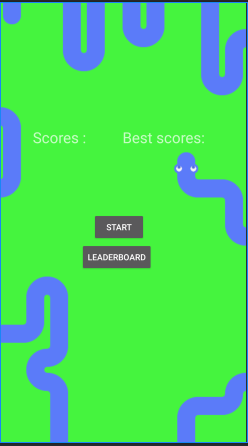
\includegraphics[scale=0.52]{Menu.png}
        \caption{Desing et blueprint du layout de l'activité \textit{ListeBestScores}}
        \label{fig:DLBS}
    \end{minipage} \hfill
    \begin{minipage}[c]{.3\linewidth}
        \centering
        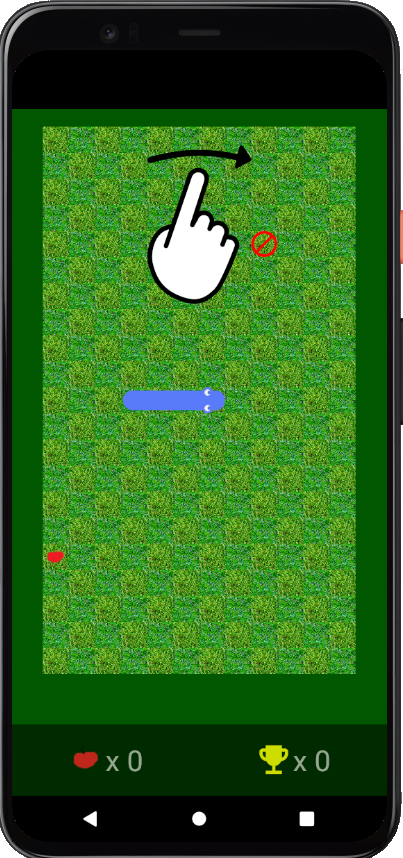
\includegraphics[scale=0.3]{Jeu.png}
        \caption{Activité \textit{ListeBestScores}}
    \end{minipage}
    \hfill
    \begin{minipage}[c]{.3\linewidth}
        \centering
        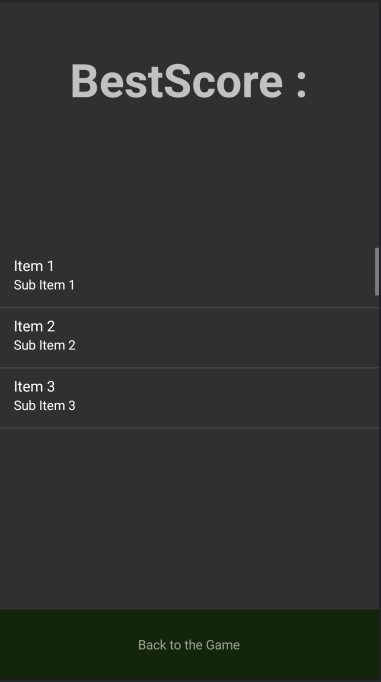
\includegraphics[scale=0.35]{ListeBestScore.png}
        \caption{Activité \textit{ListeBestScores}}
    \end{minipage}
\end{figure}

% \ref{...} permet de faire référence à un élément défini
% ailleurs dans le document (voir \label{...} plus haut).
Pour chaque application nous avons réalisé des recherches sur le jeu que nous voulions créer. Ceci nous a permis de trouver des tutoriels$^\ref{and}$. Cependant nous n'avons pas réalisé la même application, nous avons décidé de modifier celle-ci, de lui ajouter notre touche et les conaissances que nous acquis durant l'UE de développement mobile.

\subsection{Logique du jeu}
Le jeu Snake est le suivant, nous avons un serpent (Snake) qui parcourt une zone de jeu et qui doit manger des pommes pour grandir. Les pommes mangées représentent le score du joueur. Si le snake sort de la zone de jeu ou qu'il entre en collision avec une partie de son corps, alors il y a Game Over. Nous avons ajouté un panneau stop qui fait mourrir le joueur s'il entre en collision avec. Ce panneau se déplace toutes les 5 secondes.\\
Pour réaliser la zone de jeu, nous avons construit un tableau qui $lignes~\times~colonnes$ textures d'herbe qui seront dessinées dans un Canvas. Nous avons utilisé deux textures différentes pour créer un damier.\\
Comme ce Canva représente notre zone de jeu, pour que le serpent meurent en sortant de la zone de jeu. Nous devons simplement chercher quand est ce que les coordonées de la tête sont supérieures, ou inférieures à celles des textures d'herbe qui se trouvent sur les bords. Pour ce faire, testons la position de la tête à chaque update. Si ses coordonnées sont inférieurs à celles de la première texture ou supérieures à celles de la dernière texture d'herbe, alors nous appelons la fonction gameOver, qui provoque l'arrêt du jeu et affiche votre score avec le meilleur score enregistré.\\
Durant la partie, si le serpent passe sur la case où est posée une pomme, alors le score s'incrémente de 1, si le score est supérieur au meilleur score, alors celui-ci est remplacé. Si le serpent entre en collision avec le panneau stop, de la même manière qu'avec une pomme, cette fois-ci le joueur meurt et la fonction gameOver est appelée.

\newpage

\subsection{La zone du jeu}
Cette zone est construire avec des textures d'herbes. Nous avons deux textures d'herbes. Nous créeons un tableau qui contiendra les $lignes~\times~colonnes$ textures. Nous dessinons ensuite ces textures dans un Canvas.

\subsection{Le menu}
Pour notre menu, nous avons créé une nouvelle activité. A l'aide de différents boutons redirigeant vers les différentes activités que nous avons crée (Le jeu et Le tableau des scores), nous avons rendu le déplacement entre activité possible. Nous avons aussi afficher sur notre menu le dernier score obtenu ($\ne$0), ainsi que le meilleur score de la session.
\begin{figure}[H]
    \centering
    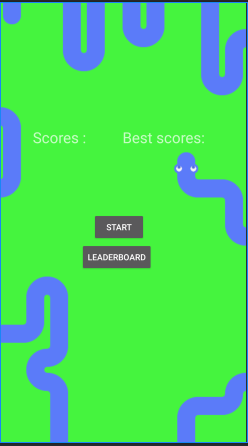
\includegraphics[scale=0.4]{Menu.png}
    \caption{Menu de l'application}
    \label{fig:menu}
\end{figure}

\subsection{La sauvegardes des meilleurs scores}
Pour ce jeu nous ne sauvegardons que les meilleurs. Pour se faire nous utilisons deux systèmes de sauvegardes. Le premier, les shared preferences qui ne gardent en mémoire qu'une petite taille de données. Nous ne gardons ici que le dernier meilleur score enregistré. Nous voulons pouvoir réaliser un historique des meilleurs scores enregistrés. Ceux ci sont enregistrés dans un fichier texte. Nous stockons dans une ArrayList<String> tous ceux que nous alons stockés. Cette liste est mise à jour à chaque fin de partie, si le score est supérieur au meilleur score d'avant la partie (celui qui apparait durant la partie et qui est à battre), alors ce score est ajouté à notre liste. \`A chaque fois que la fonction gameOver est appelée, cette liste est écrite dans un fichier qui sera lu à la prochaine ouverture de l'application.

\subsection{Affichage de la liste des meilleurs scores}
Nous affichons la liste des meilleurs stockés dans une nouvelle activité, sous une forme de liste. Pour construire la liste dans cette activité, nous avons utilisé une vue $ListView^\ref{list}$, il permet d'afficher une liste. Dans la classe de l'activité on crée un $ArrayAdapter$, il prends en argument le context de l'activité, le layout des cellules, et la liste à afficher. Ici c'est la liste des score qui est un attribut de la classe \textit{GameView}.
\begin{figure}[H]
    \centering
    \begin{minipage}[c]{.4\linewidth}
        \centering
        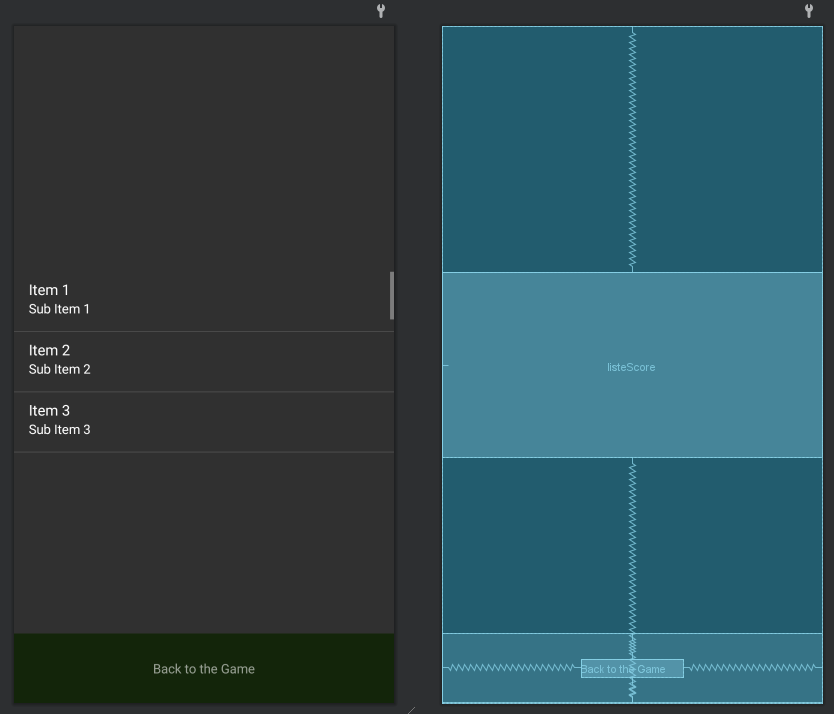
\includegraphics[scale=0.3]{DesingListeBestScores.png}
        \caption{Desing et blueprint du layout de l'activité \textit{ListeBestScores}}
        \label{fig:DLBS}
    \end{minipage} \hfill
    \begin{minipage}[c]{.4\linewidth}
        \centering
        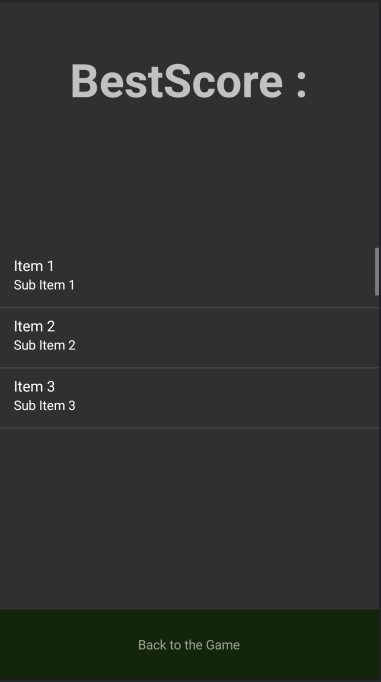
\includegraphics[scale=0.33]{ListeBestScore.png}
        \caption{Activité \textit{ListeBestScores}}
    \end{minipage}
\end{figure}

\subsection{Passage entre les activités}
Nous avons plusieurs activités dans cette application qui ont chacune un rôle. On démarre sur l'activité principale, le menu, sur ce menu, un bouton permet de lancer le jeu. L'appui sur le bouton \textit{start} démarre une nouvelle activité grâce à un \textit{Intent}. Ensuite on peut soit lancer le jeu, soit revenir au menu. Dans le menu, nous pouvons aussi accéder au tableau des meilleurs scores. C'est aussi une nouvelle activité. Dans cette activité nous affichons simplement la liste des scores qui ont battu les précédents meilleurs scores.\\
Pour changer d'activité, nosu avons utilisé deux méthodes. Nous avons placé un listener, soit sur un bouton, comme c'est le cas dans le menu, soit sur \textit{RelativeLayout}.\\
Les listener placés sur les boutons du menu permettent de lancer un nouvelle activité, en l'occurence le jeu ou le tableau des meilleurs score.\\
Alors que les listener placé dans le dialogue du jeu, ou dans le tableau des scores, terminent l'activité en cours. Ils ne relancent pas l'activité principale. Ils font appels à la fonction \textit{finish()} qui permet d'arrêter une activité.
\begin{figure}[H]
    \centering
    \begin{minipage}[c]{.4\linewidth}
        \centering
        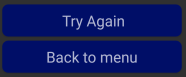
\includegraphics[scale=1]{LayoutChangeActi.png}
        \caption{\textit{RelativeLayout} de changement d'activité}
    \end{minipage} \hfill
    \begin{minipage}[c]{.4\linewidth}
        \centering
        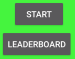
\includegraphics[scale=1.3]{ButtonsChangeActi.png}
        \caption{\textit{Buttons} de changement d'activités}
    \end{minipage}
\end{figure}

\subsection {Les Assets}
Nous avons pu récupérer plusieurs assets via les tutoriels que nous avons suivi, tel que notre image de Serpent, ou encore des assets libre de droit comme nos texture d'herbe. Nous avons aussi crée certaines de nos assets : le menu de mort (très beau), la pomme et les assets sonore enregistré directement avec le micro de notre ordinateur (Maxime TRITON pour la voix de mort).

\newpage

\section{iOS} %% une autre sous-section
Pour la partie iOS, il est important de noter que notre équipe s'est avant tout pencher sur la création d'un jeu snake sur ce système d'exploitation. N'étant pas familier avec le langage \textit{Swift} et la façon de créer une application sur Xcode, nous avons choisi de nous documenter, nous avons trouvé un tutoriels$^\ref{ios}$ que nous avons décidé de suivre.

\subsection{Logique du jeu}
Comme pour notre application sous Android, le but du jeu est de manger le plus de pommes pour faire grandir notre snake.
Cependant ici nous n'avons pas pu implémenter de façon de mourir. Nous pouvons donc sortir de la zone de jeu et revenir dans celle-ci.\\
Nous nous déplaçons à l'aide des quatre boutons placés en bas.\\
Le snake est un tableau de \textit{SnakeCell}. Une \textit{SnakeCell} est une instance d'une classe qui possède les attributs \textit{col} et \textit{row}. Ce sont des \textit{Integer} qui représente la colonne et la ligne dans laquelle se trouve cette partie du Snake. 

\subsection{La zone de jeu}
La zone du jeu a été dessinée et non créée à l'aide de textures, nous avons une view dans laquelle nous avons dessiné $lignes~\times~colonnes$ carrés depuis une origine $(x,y)$.

\subsection{Menu}
Nous avons commencer par créer une nouvelle UIViewController nous permettant d'obtenir un écran suplémentaire afin d'implémenter un menu à notre jeu déjà existant. Notre menu nous ramène comme pour notre application Android vers notre jeu à l'aide d'un bouton.

\subsection{Passage entre les activités}
Le déplacement entre activités (ici ViewController), vu traité à l'aide d'un bouton de redirection. La gestion de déplacement a été geré par \textit{self.performSegue} qu'on utilise pour rediriger vers le ViewController désiré.


\section{Contraintes}
Nous avons rencontré différents contraintes et problèmes. Nous n'avons pas eu l'occasion de travailler suffisamment sur l'application IOS. Une de nos contrainte fut d'abord dû à notre emplois du temps. \"Etant donné que Tristan est en bilicence, nous avons eu quelques soucis à nous rejoindre au PTU afin de travailler sur la version iOS de notre projet (de même pour le couvre feux). La contrainte la plus importante fut le temps. Nous avons changer de sujet de projet assez proche de l'échéance, ce qui nous a obligé à nos focaliser sur le langage nous permettant de travailler dans les meilleurs conditions. Nous avons tout de même tenté de retranscrire une version non terminé de notre Application Android sous iOS.

\section{Bugs}
Notre projet Android, bien que fonctionnel ne peut toujours pas être considéré comme terminé. Nous avons encore certains bugs que nous n'avons tout simplement pas eu le temps de résoudre. L'activité Leaderboard fait crash l'application si elle est lancé avant qu'un partie soit joué (donc qu'il y ai une valeur ajouté par le joueur inscrit). La gestion de la rotation n'est pas effectué. Le menu de mort s'affiche alors qu'on lance pour la première fois le jeu.
\section{Conclusion}
Pour conclure, nous avons crée un jeu "Snake" fonctionnel sur Android, retenant les meilleurs scores et possédant plusieurs activités. Nous avons 2 versions de snake sur iOS une version retranscrite d'Android et une version basé sur un différent systeme.

%%% La bibliographie:
\begin{thebibliography}{9}
    \bibitem{ListView}
    \label{list}
    Le Tutoriel de Android ListView
    \url{https://devstory.net/10435/android-listview}
    
    \bibitem{IOS}
    \label{ios}
    Snake on Swift iOS - YouTube
    \url{https://www.youtube.com/playlist?list=PLhct0hTlSsNn_508kHtiH8ZRUfBe6EVgt}
    
    \bibitem{android}
    \label{and}
    Snake Game With Android Studio - YouTube
    \url{https://www.youtube.com/playlist?list=PLx-Q7RE4RIUEyktbIoeRNtCryYP07OWDM}
\end{thebibliography}
\end{document}
